\documentclass[12pt,letterpaper]{article}



%%
%% Required packages:
%%
\usepackage{etex}
\usepackage{amsmath}
\usepackage{amssymb}
\usepackage{amstext}
\usepackage{amsthm}
\usepackage{fancyhdr,fancybox}
\usepackage{mathrsfs} % need for \mathscr command
\usepackage{multicol}
\usepackage[normalem]{ulem}
%\usepackage{pictex,pictexplus}
% \usepackage{pictexwd}
\usepackage{rotating}
\usepackage{url}
\usepackage{xfrac}
\usepackage{booktabs}
\usepackage{color,soul}
\usepackage{comment}

\usepackage{hyperref}
\hypersetup{
    colorlinks=true,     % false: boxed links; true: colored links
    linkcolor=blue,      % color of internal links
    citecolor=blue,      % color of links to bibliography
    filecolor=blue,      % color of file links
    urlcolor=blue        % color of external links
}


\usepackage{tikz}
\usetikzlibrary{backgrounds,calc}

%%
%% Common formatting commands
%%
\setlength{\parindent}{0in}
\setlength{\textwidth}{7in}
\setlength{\evensidemargin}{-0.25in}
\setlength{\oddsidemargin}{-0.25in}
\setlength{\parskip}{.5\baselineskip}
\setlength{\topmargin}{-0.5in}
\setlength{\textheight}{9in}

%               Problem and Part
\newcounter{problemnumber}
\newcounter{partnumber}
\newcounter{subpartnumber}
\newcommand{\Problem}{%
  \refstepcounter{problemnumber}%
  \setcounter{partnumber}{0}%
  \setcounter{subpartnumber}{0}%
  \item[\makebox{\hfil\textbf{\theproblemnumber.}\hfil}]%
  }
\newcommand{\InProblem}[2][1.6]{%
  \refstepcounter{problemnumber}%
  \setcounter{partnumber}{0}%
  \setcounter{subpartnumber}{0}%
  \textbf{\theproblemnumber.}\ \ \parbox[t]{#1in}{#2}%
}
\newcommand{\InSmallProblem}[1]{\InProblem[1.05]{#1}}
\newcommand{\NoProblem}[1]{%
  \mbox{\hfil\textbf{#1}\hfil}%
  }
\newcommand{\UnProblem}{%
  \refstepcounter{problemnumber}%
  \setcounter{partnumber}{0}%
  \setcounter{subpartnumber}{0}%
  \mbox{\hfil\textbf{\theproblemnumber.}\hfil}%
  }
\newcommand{\InFlexProblem}[1]{%
  \refstepcounter{problemnumber}%
  \setcounter{partnumber}{0}%
  \setcounter{subpartnumber}{0}%
  \textbf{\theproblemnumber.}\ \ #1%
}
%%  Part:
\newcommand{\Part}{%
  \renewcommand{\thepartnumber}{(\alph{partnumber})}%
  \refstepcounter{partnumber}
  \setcounter{subpartnumber}{0}%
  \item[(\alph{partnumber})]%
}
\newcommand{\InPart}[2][1.75]{%
  \renewcommand{\thepartnumber}{(\alph{partnumber})}%
  \refstepcounter{partnumber}%
  \setcounter{subpartnumber}{0}%
  (\alph{partnumber})\ \ \parbox[t]{#1in}{#2}%
}
\newcommand{\UnPart}{%
  \refstepcounter{partnumber}%
  \renewcommand{\thepartnumber}{(\alph{partnumber})}%
  \setcounter{subpartnumber}{0}%
  (\alph{partnumber})%
}
\newcommand{\InLargePart}[1]{\InPart[3.05]{#1}}
\newcommand{\InFullPart}[1]{\InPart[6.2]{#1}}
\newcommand{\InSmallPart}[1]{\InPart[1.05]{#1}}
%% SubPart:
\newcommand{\SubPart}{%
  \refstepcounter{subpartnumber}%
  \item[(\roman{subpartnumber})]%
  }
\newcommand{\InSubPart}[2][2.25]{%
  \stepcounter{subpartnumber}%
  (\roman{subpartnumber})\ \ \parbox[t]{#1in}{#2}%
}
\newcommand{\InSmallSubPart}[1]{\InSubPart[1.5]{#1}}
\newcommand{\InTinySubPart}[1]{%
  \stepcounter{subpartnumber}%
  (\roman{subpartnumber})\ \ \makebox{#1}%
}
\newcommand{\InMySubPart}[2][2.25]{%
  \stepcounter{subpartnumber}%
  \parbox[t]{#1in}{\makebox[0.3in][l]{(\roman{subpartnumber})}\ \ {#2}}%
}
\newcommand{\TrueFalse}{\textbf{T}\ \ \textbf{F}\ \ }
\newcommand{\TFPart}[1]{% 
  \stepcounter{partnumber}%
  \setcounter{subpartnumber}{0}%
  \item[(\alph{partnumber})] \TrueFalse\parbox[t]{5.5in}{#1}}

\newcommand{\Points}[1]{(#1 points) \ }
\newcommand{\Point}[1]{(#1 point) \ }


%% For Answers:
\newcounter{answernumber}
\newcommand{\Answer}{%
  \refstepcounter{answernumber}%
  \setcounter{partnumber}{0}%
  \setcounter{subpartnumber}{0}%
  \item[\makebox{\hfil\textbf{\theanswernumber.}\hfil}]%
  }


% Setting up the headers for the first page
%\chead{} % will default to what is typed in the file.
\fancyhead[L]{\textsc{Math 22a}}
\fancyhead[R]{\textsc{Fall 2024}}
\fancyfoot[R]{
	\vspace*{\fill}\footnotesize\textcopyright{} \emph{Harvard Math 22a}	
}
\renewcommand{\headrulewidth}{0pt}

%\fancyhead[C]{}
%	\chead{}	
%	\lhead{}
%	\rhead{}
%	\cfoot{}


% Putting copyright on the footer of each page
%\fancypagestyle{secondpage}{
%	\fancyhead[C]{TESTing again} % change this to be blank
%		%\chead{}	
%	\fancyhead[L]{bears} % change this to be blank
%	\fancyhead[R]{dogs} % change this to be blank
%	\fancyfoot[R]{ %keeps the footer the same
%		\vspace*{\fill}\footnotesize\textcopyright{} \emph{Harvard Math 22a}	
%	}
%}
%\renewcommand{\headrulewidth}{0pt}
%\pagestyle{fancy}
\pagestyle{empty}


%\lhead{}
%\rhead{}
%\rfoot{\vspace*{\fill}\footnotesize\textcopyright{} \emph{Harvard Math 22a}}
%\renewcommand{\headrulewidth}{0pt}
%\pagestyle{fancy}




%%
%% Common shortcut commands:
%%
\newcommand{\ds}{\displaystyle}
\newcommand{\sgn}{\operatorname{sgn}}
\renewcommand{\Pr}{\operatorname{P}}
\newcommand{\CPr}[3][{}]{\Pr_{\text{#1}}\left(#2\,|\,#3\right)}

\newcommand{\C}{\mathbb{C}}
\newcommand{\R}{\mathbb{R}}
\newcommand{\Z}{\mathbb{Z}}
\newcommand{\N}{\mathbb{N}}
\newcommand{\Q}{\mathbb{Q}}
\newcommand{\D}{\mathbb{D}}

\newcommand{\rref}{\operatorname{rref}}
\newcommand{\im}{\operatorname{im}}
\newcommand{\rank}{\operatorname{rank}}
\newcommand{\diag}{\operatorname{diag}}
\newcommand{\Span}{\operatorname{span}}
%\renewcommand{\vec}[1]{\mathbf{#1}}
\newcommand{\charpoly}{\mathscr{P}}
\newcommand{\nicefrac}[2]{\sfrac{#1}{#2}} % using xfrac package
\newcommand{\topology}{\mathcal{T}}
\newcommand{\Inn}{\operatorname{Inn}}

\newcommand{\blankbox}[2]{\fbox{\rule{#1}{0in}\rule{0in}{#2}}}

\newenvironment{myindentpar}[1]%
 {\begin{list}{}%
         {\setlength{\leftmargin}{#1}
          \setlength{\rightmargin}{\leftmargin}}%
         \item[]%
 }
 {\end{list}}
\newtheorem{theorem}{Theorem}
\newtheorem*{NStheorem}{Theorem}
\newtheorem{cor}[theorem]{Corollary}
\newtheorem*{claim}{Claim}
\newtheorem{defn}{Definition}

\newenvironment{amatrix}[1]{%
  \left(\begin{array}{@{}*{#1}{c}|c@{}}
}{%
  \end{array}\right)
}

%--------grstep
% For denoting a Gauss' reduction step.
% Use as: \grstep{\rho_1+\rho_3} or \grstep[2\rho_5 \\ 3\rho_6]{\rho_1+\rho_3}
\newcommand{\grstep}[2][\relax]{%
   \ensuremath{\mathrel{
       {\mathop{\longrightarrow}\limits^{#2\mathstrut}_{
                                     \begin{subarray}{l} #1 \end{subarray}}}}}}
\newcommand{\swap}{\leftrightarrow}


\usetikzlibrary{arrows}
\usepackage{wrapfig}


\chead{\Large\textbf{More Joy of Sets,  \fbox\S 14}}% 

\begin{document}
\thispagestyle{fancy}

%Recall from last class:
%
%\begin{itemize}
%\item An $n$ by $n$ matrix $A$ is {\bf invertible} if there is an $n$ by $n$ matrix $C$ so that $AC=I_n$ and $CA=I_n$. We denote the inverse of $A$ by $A^{-1}$.
%\item {\bf Theorem:} Let $A=\begin{bmatrix} a & b \\ c & d\\ \end{bmatrix}$. If $ad-bc\neq 0$, then $A$ is invertible  and $A^{-1}= \frac{1}{ad-bc} \begin{bmatrix} d & -b\\ -c &a \\ \end{bmatrix}.$
%\item We define the {\bf determinant} of $A=\begin{bmatrix} a & b \\ c & d\\ \end{bmatrix}$, denoted by $\text{det}(A)$, by $\text{det}(A)=ad-bc.$
%\end{itemize}
%
%\newpage

Let $S$ be a non-empty set.

\begin{defn}
A set $S$ is {\bf finite} if there exists a bijection (one-to-one correspondence) $f: S \to \{1, 2, \dots, n\}$ for some natural number $n$. The set $S$ is {\bf infinite} if no such bijection exists for any $n$. 
\end{defn}

{\bf Remark:} We also call the empty set finite.

\begin{defn}
The {\bf size} or {\bf cardinality} of a finite set $S$ is the unique $n$ such that there exists a bijection from $S$ to $\{1, 2, \dots, n\}$. We denote the cardinality of $S$ by $|S|$.
\end{defn}

{\bf Remark:} We also define the cardinality of the empty set to be 0.

\begin{enumerate}

\Problem 
We've seen the formula
\begin{equation*}
	|A\cup B| = |A| + |B| - |A\cap B|.
\end{equation*}
Find a formula for $|A\cup B\cup C|$.  

\vfill

\Problem Can you conjecture a more
general formula for $|A_1 \cup A_2 \cup \cdots \cup A_k|$?
\vfill

\newpage

\begin{defn}
Sets $A$ and $B$ {\bf have the same cardinality} if there is a bijection from $A$ to $B$.
\end{defn}

\Problem How do the sets $\mathbb{N}$ and $2\mathbb{N}=\{2n: n\in \mathbb{N} \}$ compare?

\vfill

\Problem How do the sets $\mathbb{N}$ and $\mathbb{N}^2$ compare?

\vfill

\begin{defn}
An infinite set $S$ is called {\bf countably infinite} if there is a bijection from $S$ to $\mathbb{N}$; otherwise $S$ is {\bf uncountably infinite} or {\bf uncountable}.
\end{defn}

\newpage

\Problem Is the set $\mathbb{Z}$ countably infinite?

\vfill

\Problem Compare the following sets.
\Part $A=(0,\infty)$ and $B=\mathbb{R}$.
\vfill
\Part $A=(0,1)$ and $B=\mathbb{R}$.
\vfill

\newpage

\Problem Compare $\mathbb{R}$ and $\mathbb{N}$.

\newpage

\begin{defn}
Define the {\bf power set} of a set $A$ as the set of all subsets of $A$; namely
$$P(A)=\{ X : X \subseteq A\}.$$
\end{defn}

\Problem Let $A=\{1,2\}$. Find the power set of $A$.

\vfill

\Problem What is $|P(\{1, \dots, n\}|$?

\vfill
\vfill
\vfill
\vfill

\newpage

{\bf Theorem:} There is no bijection from $A$ to $P(A)$.

\Problem Prove the Theorem.

\end{enumerate}


\end{document}

\newpage
\chead{\Large\textbf{More on sets -- Answers / Solutions}}%
\lhead{}
\rhead{}
\thispagestyle{fancy}

\begin{enumerate}
  \Answer The idea of 
  \begin{equation*}
    |A\cup B| = |A| + |B| - |A\cap B|
  \end{equation*}
  is that, in counting the elements of $A\cup B$, we double-count the
  elements that are in both $A$ and $B$.  That is, we double-count
  $A\cap B$.  

  With three sets the idea is similar, and we get 
  \begin{equation*}
    |A\cup B \cup C|
    = |A| + |B| + |C|
    - |A\cap B| - |A\cap C| - |B\cap C|
    + |A \cap B \cap C|.
  \end{equation*}
  Here is a pictorial representation of this that could help you come
  to grips with this formula:
  % From http://www.texample.net/tikz/examples/venn-diagram/, suitably modified:
  \newcommand{\firstcircle}{(0,0) circle (1.5)}
  \newcommand{\secondcircle}{(1,1.5) circle (1.5)}
  \newcommand{\thirdcircle}{(2,0) circle (1.5)}
  \begin{center}
    \begin{tikzpicture}[x=10mm,y=10mm]
      \fill[red,fill opacity=0.5] \firstcircle;
      \fill[blue,fill opacity=0.5] \secondcircle;
      \fill[yellow,fill opacity=0.5] \thirdcircle;
      \draw[thick] \firstcircle;
      \node[below left] at ({1.5*cos(225)},{1.5*sin(225)}) {$A$};
      \draw[thick] \secondcircle;
      \node[above] at (1,3) {$B$};
      \draw[thick] \thirdcircle;
      \node[below right] at ({2+1.5*cos(-45)},{1.5*sin(-45)}) {$C$};
    \end{tikzpicture}
  \end{center}
  One way to think about the count is to check each piece.  For
  example, if $x\in A\cap B$ but $x\not\in C$, then $x$ is counted
  positively in $|A|$ and $|B|$ and negatively in $|A\cap B|$.
  Thus $x$ is counted a total of once.  Elements in every region are
  similarly counted only once, as you can check.
  \bigskip

\Answer  The general expression is called the 
  \href{https://en.wikipedia.org/wiki/Inclusion\%E2\%80\%93exclusion_principle}{principle of inclusion-exclusion},
  and the general formula we're looking for can be formulated as
  \begin{equation*}
    |A_1 \cup A_2 \cup \cdots \cup A_k|
    = \sum_{k=1}^{n} (-1)^{k+1} \left( \sum\limits_{i_1 < i_2 < \cdots < i_k} |A_{i_1} \cap A_{i_2} \cap \cdots \cap A_{i_k}| \right).
  \end{equation*}
  Hopefully the name makes sense: we're including regions (but thus
  over-counting), then excluding regions (thus \emph{under}-counting),
  and so on until the sum is correct.  The Wikipedia article (linked
  above) has a nice diagram that shows the number of times each region
  is counted at each step in computing $|A\cup B\cup C|$.  We try to
  reproduce it here: 
  % \newcommand{\firstcircle}{(0,0) circle (1.5)}
  % \newcommand{\secondcircle}{(1,1.5) circle (1.5)}
  % \newcommand{\thirdcircle}{(2,0) circle (1.5)}
  \begin{center}
    \begin{tabular}{ccccc}
      \begin{tikzpicture}[x=7mm,y=7mm]
        \draw[thick] \firstcircle;
        \draw[thick] \secondcircle;
        \draw[thick] \thirdcircle;
        % \node[above] at (1,3) {$B$};
        % \node[below right] at ({2+1.5*cos(-45)},{1.5*sin(-45)}) {$C$};
        % A only:
        \node at ({0.35*cos(225)},{0.35*sin(225)}) {\small$1$};
        % B only:
        \node at (1,{1.5+0.35}) {\small$1$};
        % C only:
        \node at ({2+0.35*cos(-45)},{0.35*sin(-45)}) {\small$1$};
        % A and B:
        \node[xshift=-1.5mm,yshift=1.5mm] at (0.5,0.75) {\small$2$};
        % A and C:
        \node[yshift=-2.5mm] at (1,0) {\small$2$};
        % B and C:
        \node[xshift=1.5mm,yshift=1.5mm] at (1.5,0.75) {\small$2$};
        % A and B and C:
        \node[yshift=3.5mm] at (1,0) {\small$3$};
      \end{tikzpicture}
      && 
      \begin{tikzpicture}[x=7mm,y=7mm]
        \draw[thick] \firstcircle;
        \draw[thick] \secondcircle;
        \draw[thick] \thirdcircle;
        % \node[above] at (1,3) {$B$};
        % \node[below right] at ({2+1.5*cos(-45)},{1.5*sin(-45)}) {$C$};
        % A only:
        \node at ({0.35*cos(225)},{0.35*sin(225)}) {\small$1$};
        % B only:
        \node at (1,{1.5+0.35}) {\small$1$};
        % C only:
        \node at ({2+0.35*cos(-45)},{0.35*sin(-45)}) {\small$1$};
        % A and B:
        \node[xshift=-1.5mm,yshift=1.5mm] at (0.5,0.75) {\small$1$};
        % A and C:
        \node[yshift=-2.5mm] at (1,0) {\small$1$};
        % B and C:
        \node[xshift=1.5mm,yshift=1.5mm] at (1.5,0.75) {\small$1$};
        % A and B and C:
        \node[yshift=3.5mm] at (1,0) {\small$0$};
      \end{tikzpicture}
      &&
      \begin{tikzpicture}[x=7mm,y=7mm]
        \draw[thick] \firstcircle;
        \draw[thick] \secondcircle;
        \draw[thick] \thirdcircle;
        % \node[above] at (1,3) {$B$};
        % \node[below right] at ({2+1.5*cos(-45)},{1.5*sin(-45)}) {$C$};
        % A only:
        \node at ({0.35*cos(225)},{0.35*sin(225)}) {\small$1$};
        % B only:
        \node at (1,{1.5+0.35}) {\small$1$};
        % C only:
        \node at ({2+0.35*cos(-45)},{0.35*sin(-45)}) {\small$1$};
        % A and B:
        \node[xshift=-1.5mm,yshift=1.5mm] at (0.5,0.75) {\small$1$};
        % A and C:
        \node[yshift=-2.5mm] at (1,0) {\small$1$};
        % B and C:
        \node[xshift=1.5mm,yshift=1.5mm] at (1.5,0.75) {\small$1$};
        % A and B and C:
        \node[yshift=3.5mm] at (1,0) {\small$1$};
      \end{tikzpicture}
      \\
      \small
      $|A|+|B|+|C|$
      && 
      \small
      $|A|+|B|+|C|$
      && 
      \small
      $|A|+|B|+|C|$\\
      &&
      \small
      $-|A\cap B| - |A\cap C| - |B\cap C|$
      &&
      \small
      $-|A\cap B| - |A\cap C| - |B\cap C|$
      \\
      &&
      &&
      \small
      $+|A\cap B\cap C|$
    \end{tabular}
  \end{center}
  
  \Answer   Define $f: \mathbb{N} \to 2\mathbb{N}$ by $f(n)=2n$, then $f$ is a bijective. Thus the sets have the same cardinality, or $|\mathbb{N}|=|2\mathbb{N}|$.

\Answer First we give a graphical description of a bijection from $\mathbb{N}$ to $\mathbb{N}^2$. We enumerate the elements of $\mathbb{N}^2$ by starting at $(1,1)$ and moving outwards along diagonals. Using this method each pair of natural numbers is assigned a unique natural number, and hence $|\mathbb{N}|=|\mathbb{N}^2|$.


	\begin{tikzpicture}[
	scale=2,
	axis/.style={very thick, ->, >=stealth'},
	important line/.style={thick},
	dashed line/.style={dashed, thin},
	pile/.style={thick, ->, >=stealth', shorten <=2pt, shorten
		>=2pt},
	every node/.style={color=black}
	]
	% axis
	\draw[axis] (-0.1,0)  -- (4.5,0) node(xline)[right]
	{};
	\draw[axis] (0,-0.1) -- (0,4.5) node(yline)[above] {};
	
	\fill (1,1) circle (1pt);
	
	\fill (1,1) circle (1pt) node(right)[below] {$1$};
	\fill (2,1) circle (1pt) node(right)[below] {$2$};
	\fill (1,2) circle (1pt) node(right)[below] {$3$};
	\fill (3,1) circle (1pt) node(right)[below] {$4$};
	\fill (2,2) circle (1pt) node(right)[below] {$5$};
	\fill (1,3) circle (1pt) node(right)[below left] {$6$};
	\fill (4,1) circle (1pt) node(right)[below] {$7$};
	\fill (3,2) circle (1pt) node(right)[below] {$8$};
	\fill (2,3) circle (1pt) node(right)[below] {$9$};
	\fill (1,4) circle (1pt) node(right)[below] {$10$};
	
	\draw[axis] (1,1) -> (2,1);
	\draw[axis] (2,1) -> (1,2);
	\draw[axis] (1,2) -> (1,3);
	\draw[axis] (1,3) -> (2,2);
	\draw[axis] (2,2) -> (3,1);
	\draw[axis] (3,1) -> (4,1);
	\draw[axis] (4,1) -> (3,2);
	\draw[axis] (3,2) -> (2,3);
	\draw[axis] (2,3) -> (1,4);
	%\draw[axis] (4,1) -> (2,1);
	\end{tikzpicture}
	
Another approach is to define $f:\mathbb{N}^2\to \mathbb{N}$ by $f(m,n)=2^{m-1}(2n-1)$.

{\bf Claim:} Every natural number can be uniquely written as a product of an odd number and a power of 2.

\begin{proof}
If the claim fails, then there is some smallest $n$ where the claim fails. Suppose $n$ is the smallest natural number such that $n$ doesn't have a unique expression as a product of an odd number and a power of 2. If $n$ is odd, then $n$ is not divisible by 2, so $1\cdot n$ is such an expression and the only one. If $n$ is even, then consider $n/2$. Each representation of $n$ yields a corresponding representation of $n/2$, so $n/2$ is a smaller instance of the claim failing, which contradicts our assumption that $n$ is the smallest. Thus there can be no $n$ where the claim fails.
\end{proof}

Using the claim, we get that $f$ is a bijection.
  
  \Answer Yes. Recall from the problem set $g:\mathbb{Z}\to \mathbb{N}$ by $$g(k)=\begin{cases} 2k+1 & k\geq 0,\\ -2k & k<0.\end{cases}$$ We proved in the problem set that $g$ is a bijection. Thus $|\mathbb{Z}|=|\mathbb{N}|$, and hence $\mathbb{Z}$ is countably infinite.
  
  \Answer 
  
  \begin{enumerate}
  \Part Define $f: \mathbb{R} \to (0,\infty)$ by $f(x)=e^x$, then $f$ is a bijection from $\mathbb{R}$ to $(0,\infty)$.
  
  \Part Define $f: (0,1) \to \mathbb{R}$ by $f(x)=\tan \left( \pi(x-\frac{1}{2}) \right)$. We can check the function is a bijection.
  
  \end{enumerate}
  
  \Answer 
  
  {\bf Theorem:} There is no bijection from $\mathbb{N}$ to $\mathbb{R}$.
  
  \begin{proof}
  	We prove there is no biection from $\mathbb{N}$ to $(0,1)$ by contradiction. Suppose $f: \mathbb{N} \to (0,1)$ is a bijection. We express $f(n)$ as a decimal expansion (avoiding expansions ending in infinite 9's). Then
  	\begin{align*}
  		f(1)&=0.a_{11}a_{12}a_{13} \dots a_{1n} \dots\\
    	f(2)&=0.a_{21}a_{22}a_{23} \dots a_{2n} \dots\\
    	\vdots & \quad \quad\quad  \ddots\\
    	f(n)&=0.a_{n1}a_{n2}a_{n3} \dots a_{nn} \dots\\
    	\vdots &
  	\end{align*}
  Now define $b\in(0,1)$ by $b=0.b_1b_2 \dots b_n \dots $ where 
  $b_k = \begin{cases} 1 & \text{ if } a_{kk}=2,\\ 2 & \text{ if } a_{kk}\neq2.\end{cases}$ Now $f(m)\neq b$ for any $m$ since $f(m)$ and $b$ differ in the $m$-th position of their decimal expansions. Thus $f$ cannot be surjective, which contradicts our assumption that $f$ was a bijection.
  \end{proof}

This proof technique is called Cantor diagonalization. We now have $|\mathbb{R}|>|\mathbb{N}|$, and $\mathbb{R}$ is uncountable.
  
  \Answer Let $A=\{ 1,2\}$, then $P(A)=\{\emptyset, \{1\}, \{2\}, \{1,2\} \}$.
  
  \Answer 
  
  {\bf Claim:} Let $A$ be a finite set with $n$ elements, then $|P(A)|=2^n$.
  
  \begin{proof}
  We prove the claim by induction.
  
  {\bf Base Case:} When $n=1$, we have $|P(A)|=|\{\emptyset,A \}|=2^1$, and hence the base case holds.
  
  {\bf Inductive Step:} We assume if $A$ is a set with $n$ elements, then $|P(A)|=2^n$. Let $B$ be a set with $n+1$ elements; namely $B=\{b_1, \dots, b_{n+1}\}$. Let $C=\{b_1, \dots, b_n \}$, then $C$ has $n$ elements and hence there are $2^n$ possible subsets of $C$ by the induction hypothesis. Every subset of $C$ is also a subset of $B$.
  Any subset of $B$ either contains $b_{n+1}$ or not. If the subset does not contain $b_{n+1}$, then it is also a subset of $C$ and there are $2^n$ possibilities. If the subset does contain $b_{n+1}$, then it is obtained from a subset $C$ by including $b_{n+1}$. So there are $2^n$ possibile subsets containing $b_{n+1}$. Thus $|P(A)|=2^n+2^n=2^{n+1}$.
  \end{proof}
  
  \Answer 
  
  {\bf Cantor's Theorem:} There is no bijection from $A$ to $P(A)$.
  
  \begin{proof}
  	Suppose for a contradiction there is a bijection $f:A\to P(A)$. We want to show that $f$ cannot be surjective by finding a subset of $A$ that does not appear in the image of $f$. Consider $B=\{x \in A: x \not \in f(x) \}$, then $B\subseteq A$ and hence $B \in P(A)$. Since $f$ is bijective, there exists $a \in A$ such that $f(a)=B$. Now there are two possibilities $a \in B$ or $a \not \in B$.
  	
  	{\bf Case 1:} Suppose $a\in B$, then by definition of $B$, we know that $a \not \in f(a)$, which means that $a \not \in B$. Thus this case is impossible 
  	
  	{\bf Case 2:} Suppose $a \not \in B$, then $a \not \in f(a)$. Thus $a \in B$ from the definition of $B$. Thus this case is also impossible.
  	
  	Since both cases are impossible, our assumption that $f$ is bijective must be impossible.
  \end{proof}
  
\end{enumerate}

\end{document}


%%% Local ables: 
%%% mode: latex
%%% TeX-master: t
%%% End: 
